\chapter{کارهای پیشین}
\label{chapter:literature}

در این فصل به بررسی پژوهش‌های گذشته بر روی مسئله‌ی کدگذاری اندیس منعطف می‌پردازیم.

\section{مقدمه}
همان‌طور که در فصل اول گفته شد، مسئله‌ی کدگذاری اندیس منعطف توسط براهما و فرگولی در سال 2015 در
\cite{pliablefirstpaper}
به عنوان توسعه‌ای از مسئله‌ی کدگذاری اندیس معرفی شد. در این حالت هر گیرنده به جای اینکه به دنبال یک پیام خاص باشد، به دنبال یک پیام جدید است که در مجموعه‌ی اطلاعات جانبی‌ش نباشد.

این مسئله کاربردهایی مختلفی در مسائل حوزه‌های گوناگون دارد. برای مثال در محاسبات توزیع شده
\cite{datashuf}
\transf{
سیستم‌های پیشنهاد دهنده
}{recommendation system}
\cite{8404065}
\transf{
یادگیری توزیع شده
}{
distributed learning
}
\cite{8682270}.
در این فصل به مرور ادبیات پژوهشی 
\picod
می‌پردازیم.

در 
\autoref{sec:3:2}
ضمن دسته بندی مقالات این حوزه مروری اجمالی بر آن‌ها میکنیم.

در 
\autoref{sec:3:3}
به بررسی الگوریتمی تقریبی برای 
\picod
که توسط فرگولی و همکاران در
\cite{song2017polynomialtime}
معرفی شده است می‌پردازیم.
\section{
	مروری اجمالی بر مقالات حوزه
\picod
}
\label{sec:3:2}
سپس در فصل چهار با چهار گونه‌ی مختلف تعریف شده بر اساس کدگذاری اندیس منعطف آشنا خواهیم شد.
در فصل پنج به ارتباط
پس از آن مقالات متعددی روی این مسئله تمرکز کرده اند. پژوهش بر روی مسئله‌ی کدگذاری اندیس منعطف را می‌توان به دسته‌های زیر تقسیم کرد:
\begin{enumerate}
\item 
ساخت یک کد برای دسته‌ای از گراف‌ها و یا ساخت الگوریتم‌های تقریبی/تصادفی برای همه‌ی گراف‌ها
\item 
تعریف مسائل جدید بر پایه‌ی کدگذاری اندیس منعطف(مانند کدگذاری اندیس ترجیحی و ...)
\item 
استفاده از مسئله‌ی کدگذاری اندیس منعطف برای مدل سازی و حل مسائل دیگر
\item 
کران بالا برای حداکثر تعداد ارسال مورد نیاز و کران پایین برای حداقل تعداد ارسال مورد نیاز
\end{enumerate}

روی هر کدام از موضاع بالا مقالات متعددی کار کرده اند. برای مثال
\begin{enumerate}
	\item الگوریتم‌/کد جدید
	\begin{enumerate}
		\item 
		لیو در
		\cite{8278015}
		با استفاده از روش‌های نظریه اطلاعات به اثبات کران‌هایی برای چند خانواده مختلف از گراف‌های اطلاعات جانبی می‌پردازد.
		\item 
	در
	\cite{10313405}
	الگوریتمی برای.
	\item
	در
	\cite{8871209}
	مسئله را فقط برای بخشی از گراف‌های اطلاعات جانبی که
	\lr{complete–S PICOD}
	نام گذاری می‌کنند حل میکنند.
	\item
	در
	\cite{9759449}
	با تعریف یک مسئله‌ی
	\transf{
	بهینه سازی تنک و با رنک پایین}{
	sparse and low-rank optimization
	}
	و حل آن با 
	\transf{
	الگوریتم تصویر کردن تکراری
	}{Alternating Projection Algorithm}
	الگوریتمی کارا برای حل مسئله ارائه میدهند.
	\item
	در
	\cite{8682270}
	با استفاده از
	\picod
	و الگوریتم بر مبنای
	 \transf{
	 تفاوت تحدب
	 }{
	 	difference-of-convex
	 }
	 ارائه می‌دهند که بر اساس نتایج آزمایشگاهی باعث کاهش پهنای باند مورد نیاز در
	 \transf{
	 یادگیری توزیع شده روی دستگاه‌های نهایی
	 }{ON-DEVICE DISTRIBUTED LEARNING}
	 می‌شود.
	 \item
	 در
	 \cite{sasi2019pliable}
	 برای کلاس خاصی از مسئله‌ی
	 \picod
	 که
	 \transf{
	 متوالی
	 }{consecutive}
	 نامیده می‌شود بحث می‌کنند و برای دو حالت اکستریم آن کد اندیس ارائه می‌دهند. سپس در ادامه برای حالت
	 \lr{c-Constrained}
	 نیز کد ارائه می‌دهند.
	 \item 
	 در
	 \cite{8613483}
	 شبیه مقاله قبلی بر روی
	 \lr{Consecutive Complete–S}
	 کار می کنند و با استفاده از اثبات‌های ترکیبیاتی، اثباتی برای وجود کد با طول مناسب ارائه می‌دهند.
	\end{enumerate}
	 
	\item گونه‌های جدید
	\begin{enumerate}
		\item 
		لیو و همکاران در
		\cite{10015670}
		به مسئله‌ی نشتی ناخواسته‌ی اطلاعات در 
		\icod
		و
		\picod
		می‌پردازند. اگر بخشی از پیام‌ها حساس و بقیه غیر حساس باشند یک شنودکننده‌ی متخاصم بر اساس پیام‌های دریافتی چه مقدار داده کسب خواهد کرد؟ این مقدار را با
		\transf{
		نرخ نشت
		}{leakage rate}
		نشان می‌دهیم. در ادامه نرخ نشت بهینه برای مسائل
		\icod
		را اثبات می‌کنند و الگوریتم قطعی برای پیدا کردن آن ارائه می‌دهند و نشان می‌دهند نتیجه‌ی به دست آمده برای
		\icod
		برای
		\picod
		هم برقرار است.
		\item 
		فرگولی در
		\cite{6620405}
		مسئله‌ی
		\picod
		را به دو روش تعمیم می‌دهد. در روش اول هر گیرنده به جای اینکه به دنبال بازیابی یک پیام باشد به دنبال بازیابی
		$t$
		پیام است که به آن
		\lr{MULT-PICOD}
		می‌گوید.
		در روش دوم فرستنده گراف اطلاعات جالبی را در دست ندارد و تنها می‌داند که گیرنده‌ها چند پیام را از پیش به عنوان اطلاعات جانبی دارند(همه‌ی گیرنده‌ها به تعداد برابر پیام دارند.) و آن را
		\lr{OB-PICOD}
		می‌نامد.
		\item 
		لینکی کار فرگولی در مقاله قبلی را در
		\cite{8625330}
		ادامه می‌دهد و روش کدگذاری جدید برای 
		\lr{MULT-PICOD}
		ارائه می‌دهد.
		\item 
		لیو در
		\cite{9173957}
		گونه جدیدی از مسئله را تعریف میکنند که اولا به جای وجود سرور مرکزی تبادل پیام به صورت نامتمرکز انجام می‌شود  و همچنین هر گیرنده تنها یک پیام جدید خارج از اطلاعات جانبی خود بازیابی می‌کند و هیچ دیتایی راجع به بقیه پیام‌ها کسب نمی‌کند. به دلیل سختی این مسئله در ادامه تنها روی یک حالت خاص که اطلاعات جانبی گیرنده‌های به صورت
		\transf{
		جابه‌جایی های چرخشی 
		$s$
		تایی
		}{$s$ circular shifts}
		هست تمرکز می‌کنند.	

	\end{enumerate}
	\item حل مسائل دیگر
		\begin{enumerate}
			\item 
	در
	\cite{Obead_2023}
	با استفاده از  
	\picod
	مسئله‌ی
	\transf{
	بازیابی منعطف و محرمانه دیتا، همراه با اطلاعات جانبی با یک سرور
	}{
	Single-Server Pliable Private Information Retrieval With Side Information
	}
	را حل میکنند.
			\item
	سانگ و فرگولی در
	\cite{8404065}
	به ارتباط 
	\picod
	و ساختن  سیستم‌های پیشنهاد دهنده‌ با توجه به پهنای باند می‌پردازند.
	\item
	در
	\cite{e24081149}
	به ارتباط 
	\icod
	و
	\picod
	با
	\lr{error-correcting codes with multiple interpretations from the
		tree construction of nested cyclic codes}
		می پردازند.
		\item 
		فرگولی در
		\cite{datashuf}
		با استفاده از
		\picod
		به مسئله‌ی
		\transf{
			بازآرایی داده
		}{Data Shuffling}
		که در مسائل محاسبه‌ی توزیع شده ضاهر می‌شود می‌پردازد.
	\item
	\namef{لینکی}{Song, Linqi}
	و فرگولی در
	
	\cite{7176784}
	بررسی‌ای اجمالی بر تاثیر ایده‌ی فکری پشت
	\picod
	بر دسته‌ای از مسائل مخابراتی که
	\transf{
	کدگذاری نوع محتوا
	}{Content-Type Coding}
	نامیده می‌شود می پردازند. لینکی در ادامه در پایان نامه‌ی دکتری خود
	\cite{linqiphd}
	نتایج متعددی در این زمینه می‌گیرد.
		\end{enumerate}
		\item کران بالا و پایین
		\begin{enumerate}
			\item 
			کران بالای
			$\mathcal{O}(\log(n))$
			برای
			\picod
			با کران بالای
			\icod
			که
			$\mathcal{O}(n)$
			است تفاوت فاحشی دارد. لیو و تانینتی در
			\cite{7606849}
		تلاش می‌کنند با پیدا کردن کرانی برای تعداد گیرنده‌هایی که با هر پیام می‌توان ارضا کرد شهودی برای این مسئله بیابند.
			\item 
			در
			\cite{9518120}
			گراف اطلاعات جانبی را با استفاده از 
			\transf{
			هایپرگراف‌ها
			}{hyper graphs}
			مدل‌سازی کرده و کران بالایی برای تعداد ارسال‌ها پیدا میکنند. سپس با استفاده از این کران اثبات می‌کنند که برای بعضی از حالت ها کد با طول خوبی وجود دارد.
			\item
			در ادامه مقاله قبل با روش مشابه‌ای در
			\cite{9965883}
			کران بالا و کران پایین برای
			\picod
			اثبات شده است.
					\item
					\transf{انگ}{ong}
					همکاران در
			\cite{ong2019improved}
			و سپس در
			\cite{8849527}
			تکنیک بسیار متفاوتی در پیش می‌گیرند. به جای بررسی اطلاعات جانبی گیرنده‌ها به 
			\transf{
			گیرنده‌های غایب
		}{Absent Receivers}
		می‌پردازند. اگر هر گیرنده را بر اساس اطلاعات جانبیش شناسایی کنیم، به زیرمجموعه‌های مجموعه‌ی پیام‌ها که به عنوان گیرنده در گراف وجود ندارند گیرنده غایب می‌گوییم. با استفاده از این روش کران پایین جدیدی برای حداقل ارسال مورد نیاز پیدا می‌کنند.
		\end{enumerate}
\end{enumerate}


\section{
\picod
}
\subsection{تعریف دقیق مسئله}
\label{sec:3:3}
در بخش به بررسی مقالات
\cite{pliablefirstpaper,pliable2015paper,  song2017polynomialtime}
(نسخه ژرنالی مقاله دوم
\cite{7541273}
) از فرگولی و همکاران می‌پردازیم. 

	سیستمی با یک فرستنده و 
	$n$
	گیرنده در نظر بگیرید. فرستنده مقدار
	$m$
	متغیر تصادفی
	$X = (X_1, \ldots, X_n)$
	که از میدان متناهی
	$\mathcal{F}$
	را در دست دارد. هر گیرنده مانند 
	$i$
	بخشی از متغیرهای تصادفی را در اختیار دارد که اندیس آن‌ها را با 
	$S_i \subseteq [m]$
	نشان می‌دهیم. هر گیرنده می‌خواهد 
	$t$
	پیام که جز اطلاعات جانبی‌اش نیست یعنی اندیسشان در
	$R_i = [m] \setminus S_i$
	باشد را بازیابی کند.
	فرستنده می‌تواند تعدادی پیام مانند
	$Y = (Y_1, \ldots, Y_l): Y_i \in \fq$
	را برای تمام گیرنده‌ها ارسال کند تا گیرنده‌ها بتوانند با پیام‌های ارسالی و اطلاعات جانبی خود پیام‌های مورد نظر را بازیابی کنند. در
	\picod
	قبل از ارسال پیام‌ها توسط فرستنده، پیام‌هایی که توسط هر گیرنده بازیابی خواهد کرد یعنی
	$U_i \subseteq R_i,  |U_i| = t$
	 مشخص می‌شود. برعکس 
	\icod
	 که هر گیرنده پیامی مشخص را باید بازیابی کند در این‌جا مشخص کردن پیام‌هایی که بازیابی می‌شوند نیز بخشی از مسئله است.
	 
	 مسئله 
	 \picodt
	 پیدا کردن الگوریتمی است که با گرفتن 
	 $S_i$
	 ها
	 $U$
	 و
	 $Y$
	 را پیدا کند به طوری که هر گیرنده بتواند
	 $t$
	 پیام جدید را بازیابی کند و 
	 $l = |Y|$
	 کمینه شود.
	 
	 مشابه 
	 \autoref[def:icod]
	 به تعریف رسمی
	 \picodt
	 میپردازیم:
\begin{definition}[\picodt]
	\label{def:picodt}
	برای
	$n$
	و
	$m$
	و
	$S_i$
	های داده شده یک
	\picodt
	عبارت است از:
	\begin{enumerate}
		\item 
		تابع کدگذاری
		$E: \mathcal{F}^n \rightarrow \mathcal{F}^l$
		که به 
		$l$
		طول کد میگوییم.
		\item 
		توابع کدگشایی 
		$D_i: \mathcal{F}^l \times \mathcal{F}^{|S_i|} \rightarrow \mathcal{F}^t$
	\end{enumerate}
	به گونه‌ای که
	$$D_i(E(X), S_i) = (X_{\sigma_{i,1}}, \ldots, X_{\sigma_{i,t}}): \sigma_i \subseteq R_i$$
\end{definition}

در ادبیات پژوهشی به حالت
$t = 1$
،
\picod
 و به حالت
$t > 1$
حالت
\transf{
کدگذاری اندیس منعطف چند درخواسته
}{Pliable Index Coding with Multiple Requests}
می‌گویند.

\begin{remark}[
تفاوت 
\picod 
 و 
\icod
]
مسئله‌ی 
\autoref{fig:pliablefragouli1}
را در نظر بگیرید. در حالت 
\icod
 حداقل دو ارسال توسط فرستنده مورد نیاز است. ولی در
 \picod
 تنها با یک ارسال هر سه گیرنده ارضا می‌شوند.
 \begin{figure}[H]
 	\centering
 	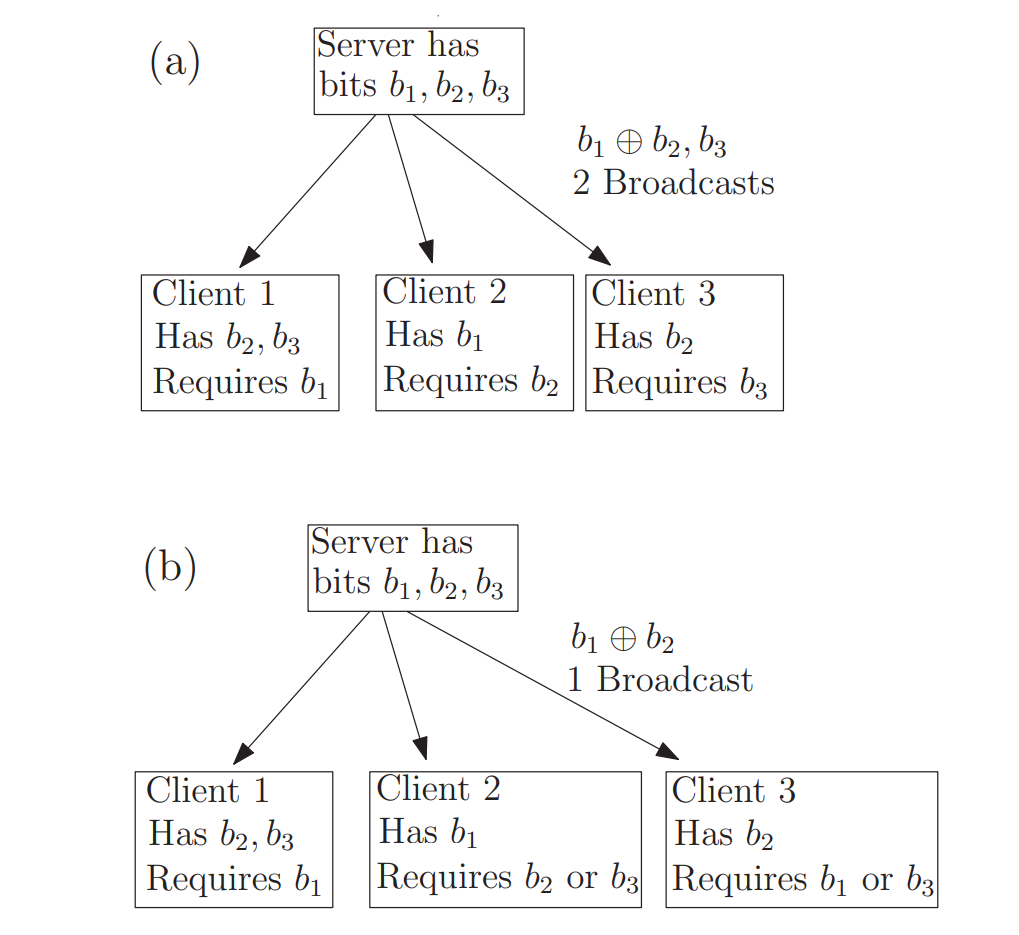
\includegraphics[width=0.6\linewidth]{figs/ch3/pliable_fragouli1}
 	\caption[
 	تفاوت
 	\icod
 	و
 	\picod
 	]{\cite{pliablefirstpaper}}
 	\label{fig:pliablefragouli1}
 \end{figure}
\end{remark}

\begin{remark}
	نکته بسیار مهمی که در ادبیات پژوهشی 
	\picod
	مخفی است و ممکن است خواننده را دچار اشتباه بسیار بزرگی کند نحوه‌ی تعریف توابع کدگشایی است. برای مثال توابع کدگشایی در
	\cite{song2017polynomialtime}
	به شکل
	$D_i: \mathcal{F}^l \times \mathcal{F}^{|S_i|} \rightarrow \mathcal{F}^t \times [m]^t$
	تعریف می‌شود، یعنی خروجی تابع
	$((X_{\sigma_1}, \sigma_1), \ldots, (X_{\sigma_t}, \sigma_t) )$
	است که به ذخن متباتر میکند که در خروجی تابع کدگشایی گیرنده‌ی 
	$i$
	ام بر اساس ورودی تابع(اطلاعات جانبی گیرنده‌ی 
	$i$
	ام و پیام‌های آن ارسال شده توسط فرستنده) مشخص می‌شود که مقدار
	$\sigma_i$
	ها چقدر است. یعنی گیرنده‌ی
	$i$
	ام بر اساس اطلاعات جانبی و پیام‌های دریافتی خود ممکن است پیام‌های مختلفی را بازیابی کند. این صورت بندی مخصوص مسئله‌ی کدگذاری اندیس بسیار منعطف است که در
	\autoref{def:verypliable}
	معرفی می‌کنیم. در مسئله‌ی
	\picod
	اگر بخواهیم به شکل کاملا دقیق توابع کدگشایی را تعریف کنیم باید 
	$\sigma$
	 را در نام تابع بیان کنیم یعنی تابع کدگشایی گیرنده‌ی
	 $i$
	 ام به شکل:
	 	$$D_{i, \sigma_i}(E(X), S_i) = (X_{\sigma_{i,1}}, \ldots, X_{\sigma_{i,t}}): \sigma_i \subseteq R_i $$
	 	در واقع زمانی که می‌خواهیم توابع کدگشایی را تعریف کنیم باید از پیش بگوییم که دقیقا کدام پیام‌ها کدگشایی خواهد شد.
\end{remark}

\begin{note}
	برای حالتی که
	$t > 1$
	است اگر
	$i$
	ای وجود داشته باشد که
	$|R_i| < t$
	در این صورت کافی است گیرنده‌ی 
	$i$
	ام
	$|R_i|$
	پیام را بازیابی کنید.
	\cite{pliablefirstpaper}
\end{note}

\begin{note}
	در 
	\cite{pliablefirstpaper}
	که اولین مقاله این موضوع است به جای استفاده از
	\picodt
	برای حالت چند درخواسته از
	\lr{$k$-\picod}
	استفاده می‌شود.
\end{note}
\begin{notation}[
	گراف اطلاعات جانبی
	]
	همان طور که در
	\autoref{notation:graph1}
	دیدم نمایش‌های گوناگوبی برای مسئله وجود دارد. در این جا ما از گراف اطلاعات جانبی استفاده می‌کنیم. همچنین به مسئله‌ی پیدا کردن کوتاه‌ترین کد اندیس منعطف برای گراف داده شده‌ی 
	$G$
	،
	\picodg
	می‌گوییم.
\end{notation}

\subsection{
\picod
،
\nphard
 است
}

\begin{lemma}
برای یک گراف
$G$
داده شده برای هر
$t$
ای همیشه
 $\text{\icodg} > \text{\picodg}$
 است.
 \cite{pliablefirstpaper}
\end{lemma}
\begin{proof}
	یک 
	\icod
	در نظر بگیرید. این کد یک
	\picod
	نیز هست. زیرا فرستنده با استفاده از همان تابع کدگذاری پیام‌ها را ارسال میکند و گیرنده‌ی
	$i$
	با استفاده از تابغ کدگشایی خود می‌تواند دقیقا	 پیام
	$i$
	ام را بازیابی کند. در واقع در
	\picod
	باید تمام حالت‌های ممکن برای بازیابی هر پیامی برای هر گیرنده را در نظر بگیریم و بین همه‌ی آن‌ها کد با کمترین طول را انتخاب کنیم که 
	\icod
	فقط یکی از آن حالت‌ها است.
\end{proof}

برای اینکه نشان دهیم
\picod 
\nphard
است، آن را به
\transf{
سه-صدق پذیری همگن یک درست
}{
MONOTONE-1in3-SAT
}
کاهش می‌دهیم.

\begin{definition}
	برای یک مصداق از مسئله‌ی 
	\transf{
	صدق پذیری
}{3SAT}
که تمام اتم‌ها بدون نقیض ضاهر شده اند، مسئله‌ی سه-صدق پذیری همگن یک درست این است که آیا یک مقدار دهی به اتم‌ها وجود دارد به صورتی که اولا عبارت را ارضا کند و دوما در هر جمله(که تمام جملات حاوی سه اتم اند) دقیقا یک اتم صادق باشد
\end{definition}

\namef{
شیفر در
}{Schaefer}
\cite{10.1145/800133.804350}
نشان می‌دهد که مسئله‌ی بالا، 
\nphard
است.

فرض کنید
$\phi$
عبارتی با اتم‌های
$\alpha_1, \ldots, \alpha_M$
و
$N_0$
جمله به شکل روبرو باشد:
$$\phi(\alpha_1, \ldots, \alpha_M) = \bigwedge\limits_{i = 1}^{N_0} CL_i, CL_i = (\alpha_{i, 1} \vee \alpha_{i, 2} \vee \alpha_{i, 3})$$

لم زیر کاهش به مسئله‌ی
\picod
را نشان می‌دهد:
\begin{lemma}
	برای یک نمونه از مسئله‌ی سه-صدق پذیری همگن یک درست مانند
	$\phi$
	یک نمونه از مسئله‌ی
	\picod
	مانند
	$I_{\phi, M, N_0}$
	وجود دارد به گونه‌ای که 
	$\phi$
	صدق پذیر است اگر و تنها اگر 
	$I_{\phi, M, N_0}$
	کدی خطی با طول یک داشته باشد.
\end{lemma}
\begin{proof}
	برای
	$\phi$
	داده شده
		$I_{\phi, M, N_0}$
		را به این شکل می‌سازیم:
		\begin{enumerate}
			\item
			$N_0$
			گیرنده
			$c_i, i \in [N_0]$
			که متناظر جمله‌ی
			$i$
			هستند.
			\item
			$M$
			متغییر تصادفی
			$b_i, i \in [M]$
			 که متناظر اتم‌ها اند.
			 \item 
			 اطلاعات جانبی گیرنده‌ی
			 $i$
			 به شکل زیر است:
			 $$S_i = {j: \alpha_j \notin CL_i}$$
			 یعنی هر گیرنده
			 $M - 3$
			 پیام را به صورت اطلاعات جانبی می‌داند.
		\end{enumerate}
		($\Rightarrow$):
		فرض کنید کدی خطی با طول یک برای
			$I_{\phi, M, N_0}$
			وجود داشته باشد. پس پیامی که فرستنده ارسال می‌کند به شکل
			$Y = (Y_1) = (b_{\sigma_1} \oplus \ldots \oplus b_{\sigma_s}), \sigma_i \in [M]$
			قرار دهید: 
			$\sigma = \{ \sigma_1, \ldots, \sigma_s \}$
			چون تمام گیرنده‌ها پیام جدیدی را با دریافت تنها یک پیام بازیابی کرده اند پس
			$\forall i \in [N_0]: \exists \sigma_t \in \sigma: \sigma_t \notin S_i$
			و چون باید بتوان با 
			$Y_1$
			دریافت شده پیامی را بازیابی کرد باید دقیقا یک
			$\sigma_t$
			به ازای هر
			$i$
			وجود داشته باشد. حال اگر در
			$\phi$
			در جمله
			$i$
			ام اتم
			$\alpha_{\sigma_t}$
			را صادق قرار دهیم تمام جملات که متناظر گیرنده‌ها هستند صادق می‌شوند و در هر جمله دقیقا یک اتم صادق است. در نتیجه یک کد خطی با طول یک را میتوان برای تولید یک مقدار دهی صادقی برای
			$\phi$
			استفاده کرد.
			
			($\Leftarrow$):
			دقیقا مشابه برهان قسمت قبلی می‌توان یک کد خطی با طول یک بر اساس یک مقدار دهی صادق است.
\end{proof}
چون سه-صدق پذیری همگن یک درست یک مسئله‌ی
\nphard
است، طبق لم قبلی 
\picod
نیز
\nphard
است.
\subsection{
الگوریتم‌های تصادفی
}
\subsubsection{
	\lr{GRCOV1} 
}
\picod
ذات بسیار متفاوتی نسبت به
\icod
دارد. مثلا زمانی که یکی از متغیرها در مجموعه‌ی اطلاعات جانبی هیچ کدام از گیرنده‌ها نباشد تنها با یک ارسال می‌توان تمام گیرنده‌ها را ارضا کرد در حالی که در
\icod
این کد با طول یک، کد درستی نیست. در واقع بر خلاف
\icod
که هر تک گیرنده ممکن است به خاطر پیامی که می‌خواهد بازیابی کند طول کد را افزایش دهد در
\picod
گیرنده‌ها برهمکنش بیشتری روی طول کد دارند. به عنوان مثالی دیگر زمانی که اطلاعات جانبی تعدادی از گیرنده‌ها شامل تمام متغیرها به جز یکی است فرشتنده کافی است مجموع تمام متغیرها را ارسال کند. 

ایده‌ی اصلی الگوریتم‌های
\lr{GRCOV1 \& GRCOV2}
 پیدا کردن مجموعه‌هایی از گیرنده‌ها است که ویژگی‌های بالا را داشته باشند.
 
 \begin{remark}
 	در مقاله
 	\cite{pliablefirstpaper}
 	نمادگذاری گراف اطلاعات جانبی بر خلاف نمادگذاری مرسوم این حوزه و این پایان نامه است. در واقع در مقالات بعدی این نمادگذاری تغییر کرد. در این مقاله اگر
 	$j \notin S_i$
 	آنگاه بین
 	$b_j$
 	و
 	$c_i$
 	یالی قرار دارد که برعکس نمادگذاری مرسوم است.
 \end{remark}
 
 فرض کنید برای دو متغیر
 $b_{\sigma_1}$
 و
 $\b_{\sigma_2}$
 \footnote{
 همان طور که در
 \autoref{remark:xbdiff}
 گفته شد 
 $b_{\sigma_1}$
 واقعا متغیر تصادفی نیست بلکه راس متناظر متغیر
 $X_{\sigma_1}$
 است.
 }
 همسایه‌های این دو راس
 $N[b_{\sigma_1}] \cup N[b_{\sigma_2}]$
 را بر اساس تعداد همسابه‌های خود در بخش
 $B$
 گراف به دو دسته تقسیم می‌کنیم. دسته اول راس‌های
 $c_i$
 ای که به همه به جز یکی وصل اند. برای مجموعه‌ی
 $B_1 \subseteq B$
 مجموعه‌ی
 $W(B_1) \subseteq C$
 تمام همسایه‌های
 $B_1$
 اند( که چون گراف دو بخشی است حتما در$C$ می‌افتند) که به 
 $|B_1| - 1$
 راس از راس‌های
 $B_1$
  وصل اند. حال اگر
  $Y_1 = \bigoplus\limits_{b \in B_1} b$
  را فرستنده ارسال کند تمام اعضای
  $W(B_1)$
  میتوانند با اطلاعات جانبی خود پیام جدیدی را با کم کردن اطلاعات جانبی خود از
  $Y_1$
  بازیابی کنند.
  
 با توجه به بحث قبلی در الگوریتم
\GRCOVone
به دنبال مجموعه‌ای از رئوس گراف مانند
$B_1$
هستیم که 
$|W(B_1)|$
بیشینه باشد. به جای اینکه در هر گام مجموعه‌ای با اندازه‌ی ماکسیمم پیدا کنیم به صورت حریضانه مجموعه‌ای با اندازه‌ی ماکسیمال پیدا می‌کنیم.

به مجموعه‌ی 
$B_1 = \{b_{v_1}, \ldots, b_{v_t}\}$
می‌گوییم ماکسیمال اگر برای هر راس
$b_{v_{t  +1}} \notin B_1$
داشته باشیم:
\begin{equation}
	\tag{شرط ماکسیمال بودن}
	|W(B_1 \cup \{b_{v_{t + 1}} \})| < |W(B_1)|
\end{equation}

برای پیدا کردن یک مجموعه‌ی ماکسیمال با یک مجموعه‌ی تهی شروع می‌کنیم و در هر گام یک راس جدید را به صورت حریصانه به طوری که 
$|W(B_1)|$
را بیشینه کند انتخاب میکنیم. این کار را تا زمانی که نتوانیم ادامه بدهیم انجام می‌دهیم.

زمانی که مجموعه‌ی ماکسیمال را پیدا کردیم مطابق آنچه قبل تر گفته شد پیام
 $Y_1 = \bigoplus\limits_{b \in B_1} b$
 را به کد خود اضافه می‌کنیم(فرستنده این پیام را هم ارسال می‌کند). سپس تمام راس‌های
 $B_1$
 و
 $W(B_1)$
 از گراف حذف می‌شوند و دوباره همین کار را تکرار می‌کنیم. در نهایت پس از 
 $s$
 گام کد نهایی برابر
 $Y = (Y_1, \ldots, Y_s), Y_i =  \bigoplus\limits_{b \in B_i} b$
 خواهد بود. این الگوریتم
 \GRCOVone\footnote{\lr{greedy cover}}
 	نام دارد. زمان اجرای این الگوریتم برابر
 	$O(mn^2)$
 	است.
 	\begin{latin}
 	\begin{algorithm}[H]
 		\caption{GrCov1($G,\alpha,\boldsymbol{\eta}$) \cite{bibid}}
 		\label{algorithm:grcov1}
 		\begin{algorithmic}[1]
 			\State Inputs: A PPICOD graph $G=(\mathbb{U}, [1:m], E, w)$ and parameters $\alpha$, $\boldsymbol{\eta}$
 			\State $\mathcal{C} \gets \emptyset$
 			\State $\mathsf{SAT} \gets \emptyset$ 
 			\While{$|\mathsf{SAT}| \neq n$}
 			\State $\textrm{maximal} \gets \code{False}$
 			\State $\mathcal{S} \gets \emptyset$
 			\While{$\textrm{maximal} = \code{False}$}
 			\State $\textrm{maximal} = \code{True}$
 			\State Randomly pick $j^* \in \arg \max_{j \in [1:m] \setminus \mathcal{S}} f(\mathcal{S} \cup \{j\})$
 			\If{$f(\mathcal{S} \cup \{j^*\}) > f(\mathcal{S})$}
 			\State $\textrm{maximal} \gets \code{False}$
 			\State $\mathcal{S} \gets \mathcal{S} \cup \{j^*\}$
 			\EndIf
 			\EndWhile
 			\State $\mathsf{SAT} \gets \mathsf{SAT} \cup W_1(\mathcal{S})$
 			\State $\mathcal{C} \gets \mathcal{C} \cup \{\mathcal{S}\}$
 			%\State \% Remove outgoing edges from $W_1(\mathcal{S})$:
 			\State $E \gets E \setminus \{ (u,v) \in E: u \in W_1(\mathcal{S})\}$
 			\EndWhile
 			\State Output: $\mathcal{C}$
 		\end{algorithmic}
 	\end{algorithm}
 	\end{latin}
 \subsubsection{
 	\lr{GRCOV2} 
 }
\subsubsection{\lr{RANDCOV}}
\subsection{الگوریتم قطعی}
\subsubsection{\lr{BinGreedy}}








